%
% 6b-regulaer.tex -- Zerlegung der regulären Darstellung
%
% (c) 2022 Prof Dr Andreas Müller, OST Ostschweizer Fachhochschule
%

%
% Zerlegung der regulären Darstellung
%
\subsection{Zerlegung der regulären Darstellung
\label{buch:gruppen:darstellung:subsection:zerlegung}}
In der regulären Darstellung einer endlichen Gruppe operiert die
Gruppe durch Translation auf den Funktionen auf $G$.
Der Charakter einer irreduzible Darstellung sowie die Matrixelemente
sind ebenfalls Funktionen auf $G$.
Es stellt sich daher die Frage, ob die Charaktere oder die Matrixelemente
irreduzibler Darstellung dazu verwendet werden können, beliebige Funktionen
auf der Gruppe im Sinne der harmonischen Analysis mit dem Skalarprodukt
für Funktionen auf der Gruppe zu konstruieren.

\subsubsection{Der Charakter der regulären Darstellung}
Der Charakter der regulären Darstellung kann direkt berechnet werden,
wie der folgende Satz zeigt.

\begin{satz}
\label{buch:gruppen:darstellung:satz:regchar}
Sei $r_G$ der Charakter der reguläre Darstellung der Gruppe $G$ auf
$\mathbb{R}[G]$, dann gilt
\begin{equation}
r_G(g)
=
\begin{cases}
|G|&\qquad\text{falls $g=e$}\\
0  &\qquad\text{sonst.}
\end{cases}
\end{equation}
\end{satz}

\begin{proof}[Beweis]
Für die Berechnung des Charakters kann eine beliebige Basis verwendet
werden.
Für die früher verwendeten Basisvektoren $v_h$ mit $h\in G$ gilt
\[
T_gv_h = v_{gh}.
\]
Da $gh=h$ nur für $g=e$ gilt, sind die Diagonalelemente der Matrix $T_g$
für $g\ne e$ alle $=0$.
Für $g=e$ ist $T_g=T_e$ in der Basis $v_h$ die Einheitsmatrix $I_{|G|}$
und damit die Spur $\tr T_e = |G|$.
Damit ist die Aussage bewiesen.
\end{proof}

Seien jetzt $\varrho_1,\dots,\varrho_h$ die irreduziblen Darstellungen
von $G$ mit Dimension $n_1,\dots,n_h$ und Charakter $\chi_i$.
Die Charaktere sind orthonormierte Funktionen, daher kann die Zerlegung
der regulären Darstellung in irreduzible Summanden mit Hilfe des
Skalarproduktes durchgeführt werden.
Da wir den Charakter der regulären Darstellung in Satz
\ref{buch:gruppen:darstellung:satz:regchar}
vollständig berechnen konnten, lässt sich jetzt auch berechnen,
dass die irreduzible Darstellung $\varrho_i$ in der reglären Darstellung
\[
\langle r_G,\chi_i\rangle
=
\frac{1}{|G|}
\sum_{g\in G} \overline{r_G(g)}\chi_i(g)
=
\frac{1}{|G|} r_G(e) \chi_i(e)
=
\frac{1}{|G|} |G| n_i
=
n_i.
\]
Die Darstellung $\varrho_i$ kommt also $n_i$ mal in der regulären Darstellung
vor.

\begin{satz}
Die reguläre Darstellung enthält jede irreduzible $n$-dimensionale
Darstellung $n$ mal.
\end{satz}

Es folgt aber noch mehr. 
Der Charakter der regulären Darstellung kann als Linearkombination
\[
r_G(g)
=
\sum_{i=1}^h \langle \chi_i,r_G\rangle \chi_i(g)
=
\sum_{i=1}^h n_i \chi_i(g)
\]
geschrieben werden.
Aus dieser Formel folgt sofort der folgende Satz.

\begin{satz}
Die Dimensionen $n_i$ der irreduziblen Darstellungen von $n$ erfüllen
\[
\sum_{i=1}^n n_i^2 = |G|
\]
Die Werte $\chi_i(g)$ der Charaktere der irreduziblen Darstellungen erfüllen
für $g\ne e$ die Relation
\[
\sum_{i=1}^n n_i\chi_i(g) = 0.
\]
\end{satz}

%
% Zerlegung der regulären Darstellung
%
\subsubsection{Zerlegung der regulären Darstellung}
Die reguläre Darstellung enthält jede irreduzible Darstellung genau
so oft, wie die Dimension angibt.
In einer geeigneten Basis ist eine solche Darstellung unitär.
Die $n^2$ Matrixelemente sind orthogonal als Funktionen auf der Gruppe.
Die Matrixelemente bilden daher einen $n^2$-dimensionalen invarianten 
Unterraum der regulären Darstellung, dies sind genau die $n$
Kopien der zugehörigen irreduziblen Darstellung.

Die reguläre Darstellung lässt sich daher in eine Blockform bringen,
die für jede Darstellung $\varrho_i$ einen $n_i^2\times n_i^2$-Block
der Form
\[
T_g
=
\left(\raisebox{-2.95cm}{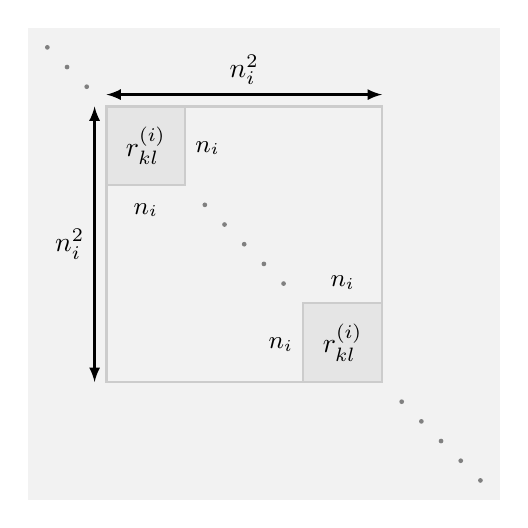
\begin{tikzpicture}[>=latex,thick]
\fill[color=gray!10] (-3,-3) rectangle (3,3);
\fill[color=gray!20] (-2,2) rectangle (-1,1);
\draw[color=gray!40] (-2,2) rectangle (-1,1);
\fill[color=gray!20] (0.5,-0.5) rectangle (1.5,-1.5);
\draw[color=gray!40] (0.5,-0.5) rectangle (1.5,-1.5);
\draw[color=gray!40] (-2,2) rectangle (1.5,-1.5);
\draw[color=gray!40] (-2,2) -- (-1.5,2);
\draw[color=gray!40] (0.5,-0.5) -- (1,-0.5);
\draw[color=gray!40] (0.5,-0.5) -- (0.5,-1);
\foreach \x in {2.75,2.5,2.25,0.75,0.5,0.25,0,-0.25,-1.75,-2,-2.25,-2.5,-2.75}{
	\fill[color=gray] (-\x,\x) circle[radius=0.03];
}
\node at (-1.5,1.5) {$r^{(i)}_{kl}$};
\node at (-1.5,1) [below] {\small $n_i\mathstrut$};
\node at (-1,1.5) [right] {\small $n_i\mathstrut$};
\node at (1,-1) {$r^{(i)}_{kl}$};
\node at (0.5,-1) [left] {\small $n_i\mathstrut$};
\node at (1,-0.5) [above] {\small $n_i\mathstrut$};
\draw[<->] (-2,2.15) -- (1.5,2.15);
\node at (-0.25,2.15) [above] {$n_i^2\mathstrut$};
\draw[<->] (-2.15,2) -- (-2.15,-1.5);
\node at (-2.15,0.25) [left] {$n_i^2\mathstrut$};
\end{tikzpicture}}
\right)
\]
enthält.
Jeder Block besteht aus $n_i$ identischen $n_i\times n_i$ Unterblöcken.
Die Matrixelemente $r^{(i)}_{kl}(g)$ dieser Unterblöcke bilden eine
orthonormierte Basis des Unterraumes der zu $\varrho_i$ isomorphen
Darstellungen in der regulären Darstellung.

\begin{beispiel}
Die zyklische Gruppe $C_n=\{0,\dots,n-1\}$ der Reste modulo $n$ hat $n$
Elemente.
Da sie abelsch ist, sind die irreduziblen Darstellungen eindimensional.
Da die Gruppe von $1$ erzeugt wird, ist die Darstellung $\varrho$ durch
das Element $\varrho(1)$ vollständig festgelegt.
Wegen $\varrho(n)=\varrho(0)=1$ muss $\varrho(n)=\varrho(1)^n =1$ sein,
d.~h.~$\varrho(1)=e^{2\pi ik/n}$ mit $k\in \{0,\dots,n-1\}$.
Die zugehörigen Funktionen auf $C_n$ sind  die Funktionen
$x\mapsto e^{2\pi ikx}$.
Aus der allgemeinen Theorie der Darstellungen folgt jetzt, dass diese
Funktionen bezüglich des Skalarproduktes
\[
\langle f,g\rangle
=
\frac{1}{n} \sum_{x=0}^{n-1} \overline{f(x)} g(x)
\]
orthonormiert sind.
Damit haben wir die Basisfunktionen der diskreten harmonischen
Analysis für die Gruppe $C_n$ aus der Darstellungstheorie wiedergewonnen.
\end{beispiel}

%
% Zerlegung der regulären Darstellung einer kompakten Lie-Gruppe
%
\subsubsection{Zerlegung der regulären Darstellung einer kompakten Lie-Gruppe}
Die Zerlegung der regulären Darstellung funktioniert auch für eine
Lie-Gruppe, was aber etwas aufwendiger zu beweisen ist.
Insbesondere ist es nicht sinnvoll, vom Charakter der regulären Darstellung
zu sprechen, da die reguläre Darstellung eine unendlichdimensionale 
Darstellung ist.
Es gilt aber weiterhin, dass endlichdimensionale irreduzible
Darstellungen genau dann isomorph sind, wenn ihr Skalarprodukt $1$ ist.
Auch die Matrixelemente einer $n$-dimensionalen irreduziblen Darstellungen
sind $n^2$ orthonormierte Funktionen, die eine Basis der $n$ in der
regulären Darstellung von $G$ vorkommenden Kopien der irreduziblen
Darstellung sind.

\begin{beispiel}
Die Gruppe $\mathbb{R}/2\pi\mathbb{Z}$ der Winkel ist abelsch.
Die Matrixelemente sind Funktionen, die unter der Translation invariant
sind, dies sind die Funktionen $x\mapsto e^{ikx}$ mit $k\in \mathbb{Z}$.
Als Skalarprodukt ist
\[
\langle f,g\rangle
=
\frac{1}{2\pi}
\int_0^{2\pi} \overline{f(x)}g(x)\,dx
\]
zu verwenden.
Die allgemeine Theorie zeigt dann, dass die Funktionen $e^{ikx}$ eine
orthonormierte Basis der integrierbaren Funktionen auf der $G$ ist.
Damit haben wir die Theorie der Fourier-Reihen aus der Darstellungstheorie
gewonnen.
\end{beispiel}




